\chapter{Lämpötila-anturi ja valoanturi}

\section{Lämpömittari}
\subsection{Lämpötila-anturin käyttöönotto}
\begin{minipage}{0.5\textwidth}
\begin{tcolorbox}[colback=lime!10,title=Tarvikkeet, colbacktitle=green!10,coltitle=black]
\begin{itemize}
    \item Lämpötila-anturi (TMP36) 
    \item Koekytkentälevy
    \item Arduino UNO 
    \item Hyppylankoja
\end{itemize}
\end{tcolorbox}
\end{minipage}
\begin{minipage}{0.5\textwidth}
\begin{tcolorbox}[colback=blue!10,title=Piirin toiminta,colbacktitle=purple!90]
Lämpötila-anturin kytkentä ja käyttö, saadun anturin arvon muuntaminen Celcius-asteiksi.
\tcblower
\begin{center}
\begin{tikzpicture}
\ctikzset{american}
%\draw (0,0) to[R,l=$220\Omega$] (0,-2) to [led] (0,-4);
\draw (-2,0) to[V,a=$5V$] (-2,-4); 
\draw (0,0) to[short] (0,-1.3);
\draw (0,-4) to[short] (0,-2.7);
\draw (0.2,-1.3) -- (-0.2,-1.3);
\draw (-0.2,-1.3)--(-0.2,-2.7);
\draw (-0.2,-2.7)--(0.2,-2.7);
\draw (0.2,-2.7) to[bend right] (0.2,-1.3);
\draw (-0.2,-2)--(-0.5,-2) to[short,-o] (-0.7,-2) node[left] {A0};
\node[text width=0.5] at (0,-2) {T M P};
\draw (-2,0) to[short] (0,0);
\draw (-2,-4) to[short] (0,-4);
\end{tikzpicture}
\end{center}
\end{tcolorbox}
\end{minipage}

\begin{tcolorbox}[colback=red!10,colbacktitle=red,title=HUOM!]
Aina kun rakennat tai muutat piiriä, pidä Arduino irrotettuna tietokoneesta! 
\end{tcolorbox}

\begin{tcolorbox}[title=Lämpötila-anturi,colback=blue!10,colbacktitle=purple!90]
Huomaa, että on merkitystä miten päin lämpötila-anturi kytketään piiriin! 

Jos tasainen sivu on kohti sinua, silloin vasemman puoleisin jalka on käyttöjännite (5V), keskimmäiseltä jalalta (A niin kuin anturi) voidaan lukea tulos ja oikean puoleisin jalka kytketään maahan (GND).

\begin{center}
\begin{tikzpicture}
\node[draw, minimum height=2,color=white,fill=black] (A) at (0,0) {TMP};
\draw[fill=black] (A.north west) to[bend left=70] (A.north east);
\draw[thick] (A.south west)++(0.1,0) --++(0,-0.5) to[short] ++(0,-.5) node[below,left] {5V};
\draw[thick] (A.south) --++(0,-0.5) to[short] ++(0,-.5) node[below] {A};
\draw[thick] (A.south east)++(-0.1,0) --++(0,-0.5) to[short] ++(0,-.5) node[below,right] {GND};
\end{tikzpicture}
\end{center}

Jos kytket anturin väärinpäin, se voi kuumentua. Ole siis tarkkana!
\end{tcolorbox}

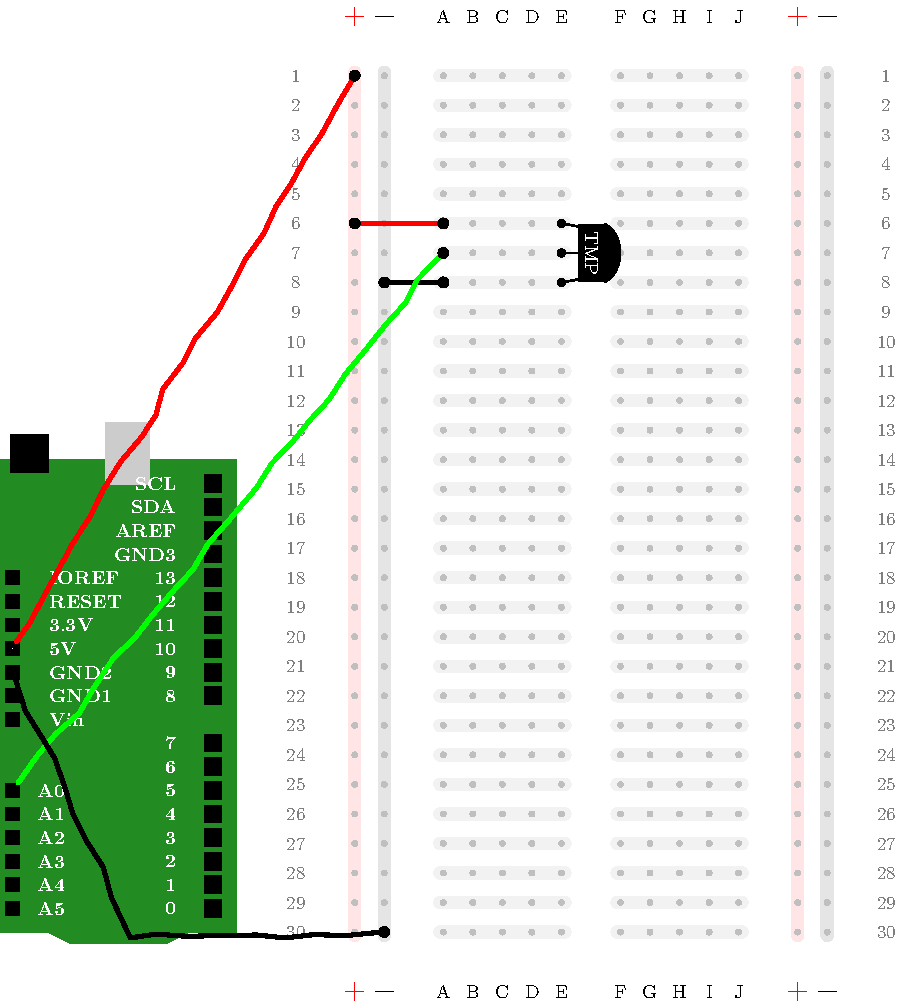
\includegraphics[width=0.8\textwidth]{kuvat/kuva12.pdf}

% \begin{tikzpicture}[scale=0.5]
% \pic[scale=0.2] at (0,0) {myarduino};
% \BREADBOARD(20,30){30};
% \coordinate[right=0.5] (tmp) at (E7);

% \node[draw,minimum height=2,color=white,fill=black] (t1) at (tmp) {\rotatebox[]{-90}{TMP}};
% \draw[fill=black] (t1.north east) to[bend left=70] (t1.south east);
% \draw[thick] (t1.north west)++(0,-0.1)  to[short,-*] (E6);
% \draw[thick] (t1.west) to[short,-*] (E7);
% \draw[thick] (t1.south west)++(0,0.1) to[short,-*] (E8);

% \draw[red,wire] (A6) to[short,*-*] (l-6);
% \draw[black,wire] (A8) to[short,*-*] (lg8);

% \draw[green,wire] (A7) to[short,*-*] (ArA0);

% %\draw[wire,red] (l-10) to[short,*-*] (A10);
% %\draw[wire,black] (lg19) to[short,*-*] (A19);
% \draw[black,wire] (ArGND2) -- ++(4,-9) to[short,-*] (lg30);
% \draw[red,wire] (l-1) to[short,*-o] (Ar5V);
% \end{tikzpicture}

\begin{tcolorbox}[colback=white,title=Vinkkejä Arduinolla koodaamiseen!,colbacktitle=purple!90]
\begin{lstlisting}
// Seuraava rivi kuuluu setup()-funktion sisalle
Serial.begin(9600); // Aloittaa kommunnikoinnin tietokoneen kanssa
// 9600 kertoo kuinka monta bittia sekunnissa lahetetaan.

// Komentoja, joilla voidaan tulostaa
Serial.print(muuttuja); // Tulostetaan muuttujan muuttuja arvo
Serial.print("Teksti:"); // Tulostetaan Teksti: 
Serial.println(muuttuja); // Sama kuin muuttujan tulostus, mutta rivinvaihto lopussa
Serial.print("\n"); // Rivinvaihto manuaalisesti
\end{lstlisting}
\end{tcolorbox}

Nämä tulostetut asiat löytyvät Arduinon "Serial Monitor":sta, eli oikean yläkulman suurennuslasi-kuvakkeen takaa.

\begin{figure}[h!]
    \centering
        \begin{tikzpicture}[remember picture]
\node (fig1) at (0,0)
       {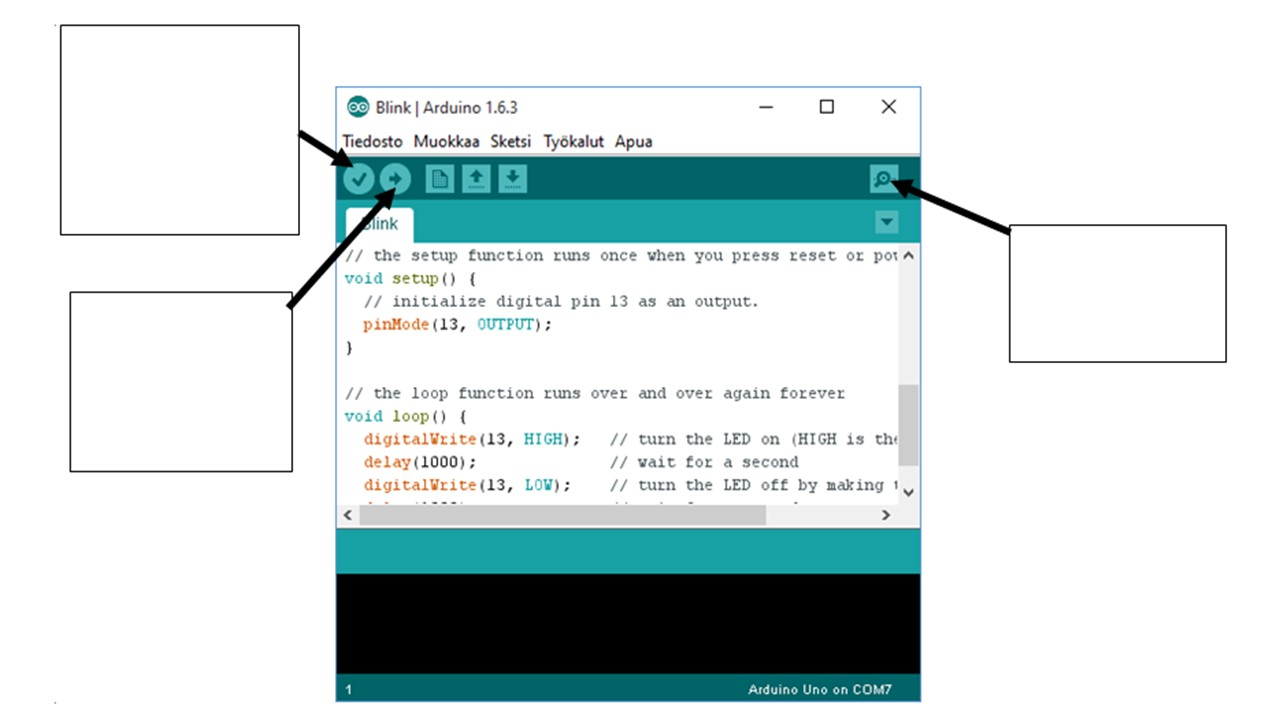
\includegraphics[scale=0.45]{kuvat/ohjelmointiymparisto.jpg}};
\end{tikzpicture}
\begin{tikzpicture}[remember picture, overlay]
       \node [align=left,] at (-5.4,7.7) {\textit{Verify/Tarkista}\\Ohjelma\\tarkistaa\\mutta ei ladata\\Arduinolle };
       \node [align=left,] at (-5.4,4.7) {\textit{Upload/Lataa}\\Ohjelma\\ladataan\\Arduinolle };
       \node [align=left,color=red] at (5.85,5.7) {Avaa sarjaportin\\monitorointi-\\ikkunaan };
\end{tikzpicture}
    %\caption{Arduinon ohjelmointiympäristö ja keskeiset hallinnointi painikkeet. }
    %\label{fig:ohjelmointiymparisto}
\end{figure}

Kopioi alla oleva koodi Arduinoon.
\begin{lstlisting}[numbers=none,showstringspaces=false] 
void setup() {
   Serial.begin(9600);
}

void loop() {
  int sensorVal = analogRead(A0); // Luetaan anturin arvo portista A0
  Serial.print("Anturin arvo: "); // lisataan selitys luvulle
  Serial.print(sensorVal); // ja tulostetaan anturin arvo
  float voltage = (sensorVal/1024.0)*5.0; // Muunna anturin arvo volteiksi
  Serial.print(". Voltteina: "); // Selitys
  Serial.print(voltage);   // Ja tulosta se
  float temp = (voltage-0.5)*100;  // Muunnetaan jannite Celcius-asteiksi
  Serial.print(". Astetta "); // Selitys
  Serial.print(temp); // ja tulostetaan lampotila
  Serial.print(" C\n"); // Celcius-astetta ja vaihdetaan rivia
  delay(1000); // Lisataan odotus, jotta ehditaan lukea tulos
}
\end{lstlisting}

\begin{tcolorbox}[colback=yellow!10, title={Lämpötila},colbacktitle=orange]
Kirjoita ylös saamasi huoneen lämpötila. Esimerkiksi 20.0 astetta.
\end{tcolorbox}

\subsection{LEDien lisääminen}\label{sec:lampo}
\begin{minipage}{0.5\textwidth}
\begin{tcolorbox}[colback=lime!10,title=Tarvikkeet, colbacktitle=green!10,coltitle=black]
\begin{itemize}
    \item Edellisen kohdan piiri rakennettuna
    \item Keltainen ja punainen LED
    \item 2 kappaletta 220$\Omega$ vastuksia:   
\includegraphics[width=0.5\textwidth]{kuvat/220.pdf}
\end{itemize}
\end{tcolorbox}
\end{minipage}
\begin{minipage}{0.5\textwidth}
\begin{tcolorbox}[colback=blue!10,title=Piirin toiminta,colbacktitle=purple!90]
Lisätään havainnointia varten kaksi LEDiä, joiden avulla saadaan tietää onko huoneessa sopivan lämpöistä, kuumaa vai liian kuumaa.
\tcblower
\begin{center}
\begin{tikzpicture}
\ctikzset{american}
\draw (0,4) to [led,l=punainen,fill=red] (0,2);
\draw (0,2) to[R,a=$220\Omega$] (0,0);
\draw (0,0) -- (0,-0.5) node[ground]{}; 
\draw (-1,4) node[left] {7} to[short,o-] (0,4);

\draw (3,4) to [led,l=keltainen,fill=yellow] (3,2);
\draw (3,2) to[R,a=$220\Omega$] (3,0);
\draw (3,0) -- (3,-0.5) node[ground]{}; 
\draw (2,4) node[left] {6} to[short,o-] (3,4);

\end{tikzpicture}
\end{center}
\end{tcolorbox}
\end{minipage}

\begin{tcolorbox}[colback=red!10,colbacktitle=red,title=HUOM!]
Aina kun rakennat tai muutat piiriä, pidä Arduino irrotettuna tietokoneesta! 
\tcblower
Muista tarkistaa miten päin LEDit kytketään! Tämä löytyy esimerkiksi sivulta \pageref{box:led}.
\end{tcolorbox}

\begin{tcolorbox}[colback=white,title=Vinkkejä Arduinolla koodaamiseen!,colbacktitle=purple!90,breakable]
\begin{lstlisting}
// Halutaan tehda monta asiaa riippuen monesta asiasta
if (ehto) {
    // Mita tehdaan jos ehto patee
} else if (ehto2) {
    // Mita tehdaan jos ehto2 patee
} else if (ehto3) {
   // Naita voit lisata niin monta kuin tarvitset
} else {
    // Ja halutessa voit maaritella myos mita tehdaan muulloin
}

// Erilaisia ehtoja
muuttuja < luku // Muuttujan muuttuja arvo on pienempi kuin annettu luku
muuttuja <= luku // Muuttujan muuttuja arvo on pienempi tai yhta suuri kuin luku
muuttuja > luku // Muuttuja on suurempi kuin luku
// Kaksi ehtoa yhta aikaa
muuttuja >= luku1 && muuttuja < luku2 // Muuttuja on suurempi tai yhtasuuri kuin luku1 JA pienempi kuin luku2
\end{lstlisting}
\end{tcolorbox}

Lisätään LEDit sekä vastukset kuvan mukaisesti.

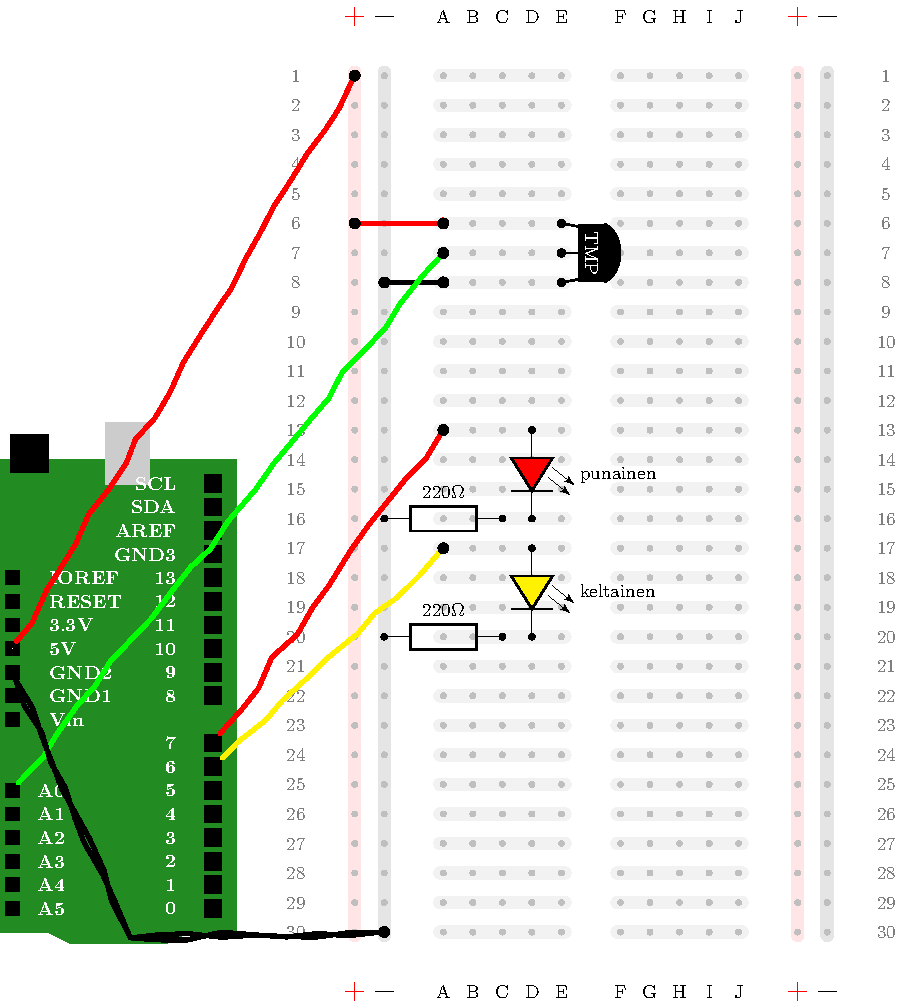
\includegraphics[width=0.8\textwidth]{kuvat/kuva13.pdf}

Lisätään koodiin LEDien ohjaaminen.

\begin{lstlisting}[numbers=none,showstringspaces=false] 
// Lisataan saatu huoneenlampo tahan
const float huoneLamp = 20.0; // Muokkaa lukua edellisen tehtavan mukaiseksi

void setup() {
Serial.begin(9600);
pinMode(7,OUTPUT); // Punainen LED on portissa 7
pinMode(6,OUTPUT); // Keltainen LED on portissa 6
}

void loop() {
  int sensorVal = analogRead(A0); // Luetaan anturin arvo portista A0
  Serial.print("Anturin arvo: "); // lisataan selitys luvulle
  Serial.print(sensorVal); // ja tulostetaan anturin arvo
  float voltage = (sensorVal/1024.0)*5.0; // Muunna anturin arvo volteiksi
  Serial.print(". Voltteina: "); // Selitys
  Serial.print(voltage);   // Ja tulosta se
  float temp = (voltage-0.5)*100;  // Muunnetaan jannite Celcius-asteiksi
  Serial.print(". Astetta "); // Selitys
  Serial.print(temp); // ja tulostetaan lampotila
  Serial.print(" C\n"); // Celcius-astetta ja vaihdetaan rivia

  // Lisataan mita tehdaan jos lampotila nousee tai laskee liikaa
  if (temp <= huoneLamp){
    // Jos huoneen lampo: sytytetaan keltainen LED
    digitalWrite(7,LOW); // Sammutetaan punainen LED tarvittaessa
    digitalWrite(6,HIGH); // Sytytetaan keltainen LED
  }else if(temp>huoneLamp+2 && temp <huoneLamp+4){
    // Lampo on nousemassa: sytytetaan molemmat valot
    digitalWrite(7,HIGH); // Sytytetaan punainen valo
    digitalWrite(6,HIGH); // Sytytetaan keltainen valo
  }else if (temp>huoneLamp+4) {
    // Lampo on noussut liikaa, varoitetaan pelkalla punaisella valolla
    digitalWrite(7,HIGH); // Sytytetaan punainen valo
    digitalWrite(6,LOW); // Sammutetaan keltainen valo
  }
  delay(1000); // Lisataan odotus, etta ehditaan lukea teksti
}
\end{lstlisting}

Nyt, avaa jälleen sarjaportin monitorointi-ikkuna. Ota kevyesti kiinni lämpötila-anturista ja katso missä vaiheessa punainen LED syttyy. Saatko myös keltaisen LEDin sammumaan? 

\begin{tcolorbox}[title=Haaste!,colback=teal!10,colbacktitle=teal!90]
Muuta koodia niin, että jos huoneessa on vähintään 2 astetta kylmempää kuin normaalisti, keltainen valo palaa. Jos huoneessa on taas normaalin lämpöistä, mikään valo ei pala. Jos huoneessa on vähintään 2 astetta lämpimämpää kuin normaalisti, punainen valo palaa.
\end{tcolorbox}

\begin{tcolorbox}[colback=yellow!10, title={Koodaa!},colbacktitle=orange,breakable]
\begin{solution}
\begin{lstlisting}
// Lisataan saatu huoneenlampo tahan
const float huoneLamp = 20.0; // Muokkaa lukua todelliseksi lampotilaksi

void setup() {
Serial.begin(9600);
pinMode(7,OUTPUT); // Punainen LED on portissa 7
pinMode(6,OUTPUT); // Keltainen LED on portissa 6
}

void loop() {
  int sensorVal = analogRead(A0); // Luetaan anturin arvo portista A0
  Serial.print("Anturin arvo: "); // lisataan selitys luvulle
  Serial.print(sensorVal); // ja tulostetaan anturin arvo
  float voltage = (sensorVal/1024.0)*5.0; // Muunna anturin arvo volteiksi
  Serial.print(". Voltteina: "); // Selitys
  Serial.print(voltage);   // Ja tulosta se
  float temp = (voltage-0.5)*100;  // Muunnetaan jannite Celcius-asteiksi
  Serial.print(". Astetta "); // Selitys
  Serial.print(temp); // ja tulostetaan lampotila
  Serial.print(" C\n"); // Celcius-astetta ja vaihdetaan rivia

  // Lisataan mita tehdaan jos lampotin
  if (temp < huoneLamp-2){
    // Huoneessa alkaa olla kylma
    digitalWrite(7,LOW); // Sammutetaan punainen LED tarvittaessa
    digitalWrite(6,HIGH); // Sytytetaan keltainen LED
  }else if(temp>=huoneLamp-2 && temp <huoneLamp+2){
    // Normaalihuoneen lampo
    digitalWrite(7,LOW); // Sytytetaan punainen valo
    digitalWrite(6,LOW); // Sytytetaan keltainen valo
  }else if (temp>huoneLamp+2) {
    // Lampo on noussut liikaa, varoitetaan pelkalla punaisella valolla
    digitalWrite(7,HIGH); // Sytytetaan punainen valo
    digitalWrite(6,LOW); // Sammutetaan keltainen valo
  }
  delay(1000); // Odotetaan, etta ehditaan lukea
}
\end{lstlisting}
Kylmemmäksi muuttumista voi olla vaikeampi havaita, varsinkin jos esimerkiksi ikkunaa ei saa auki, tai ei voida jäähdyttää sormia kylmällä vedellä. Muista, että kädet pitää kuitenkin olla kuivat, jotta voidaan koskea lämpöanturiin!
\end{solution}
\end{tcolorbox}

\clearpage
\section{Valoanturi}
\subsection{Valoanturin käyttöönotto}
\begin{minipage}{0.5\textwidth}
\begin{tcolorbox}[colback=lime!10,title=Tarvikkeet, colbacktitle=green!10,coltitle=black]
\begin{itemize}
    \item Valodiodi 
    \item Koekytkentälevy
    \item Arduino UNO 
    \item Hyppylankoja
    \item Vastus 10k$\Omega$: 
\includegraphics[width=0.5\textwidth]{kuvat/10k.pdf}
\end{itemize}
\end{tcolorbox}
\end{minipage}
\begin{minipage}{0.5\textwidth}
\begin{tcolorbox}[colback=blue!10,title=Piirin toiminta,colbacktitle=purple!90]
Valodiodin käyttö.
\tcblower
\begin{center}
\begin{tikzpicture}
\ctikzset{american}
%\draw (0,0) to[R,l=$220\Omega$] (0,-2) to [led] (0,-4);
\draw (-2,0) to[V,a=$5V$] (-2,-4); 
\draw (0,0) to[photodiode] (0,-2);
\draw (0,-2) to[R=10k$\Omega$] (0,-4);
\draw (0,-2) to[short,*-o] (2,-2) node[right] {A1};
\draw (-2,0) to[short] (0,0);
\draw (-2,-4) to[short] (0,-4);
\end{tikzpicture}
\end{center}
\end{tcolorbox}
\end{minipage}

\begin{tcolorbox}[colback=red!10,colbacktitle=red,title=HUOM!]
Aina kun rakennat tai muutat piiriä, pidä Arduino irrotettuna tietokoneesta! 
\tcblower
Voit jättää vielä edellisen kohdan piirin purkamatta! Sitä tarvitaan seuraavassa työssä. Tämän työn pystyy rakentamaan myös ilman edellisen kohdan piiriä, mutta seuraavassa työssä on käytössä sekä valo- että lämpöanturit.
\end{tcolorbox}

\begin{tcolorbox}[title=Valoanturin kytkeminen,colback=blue!10,colbacktitle=purple!90]
Huomaa, että on merkitystä kummin päin valoanturi kytketään koekytkentälevylle! 

Valoanturissa on kaksi jalkaa, joista toinen on pidempi. Valodiodi näyttää kirkkaalta LEDiltä, mutta siitä puuttuu pyöristetty yläosa, eli yläpinta on tasainen (toisin kuin LEDeillä, joilla se on pyöreä). Piirrosmerkissä nuolet tulevat kohti diodia, eli olemme ottamassa valoa sisään (emmekä lähettämässä sitä ulos kuten LEDin kanssa). 

Valoanturin muovi on toiselta puolelta kaareva, ja toiselta siinä on suora leikkaus, lyhyempi jalka on suoran leikkauksen puolella. Lyhyemmän jalan nimi on katodi ja pidemmän jalan anodi.

Piirrosmerkissä:
\begin{center}
\begin{tikzpicture}
%\node at (-1,0) {anodi};
\draw (0,0) node[left,text width=1.5cm] {anodi\\ pitkä jalka} to[photodiode,o-o] (2,0) node[right,text width=2cm] {katodi\\lyhyt jalka};
\end{tikzpicture}
\end{center}

Valodiodi kytketään myös aina vastuksen kanssa sarjaan, nyt käytössä on 10k$\Omega$ vastus. 
\end{tcolorbox}

\clearpage
Huomaa, että lisäsimme käyttöön myös oikealle puolelle käyttöjännitteen ja maan.

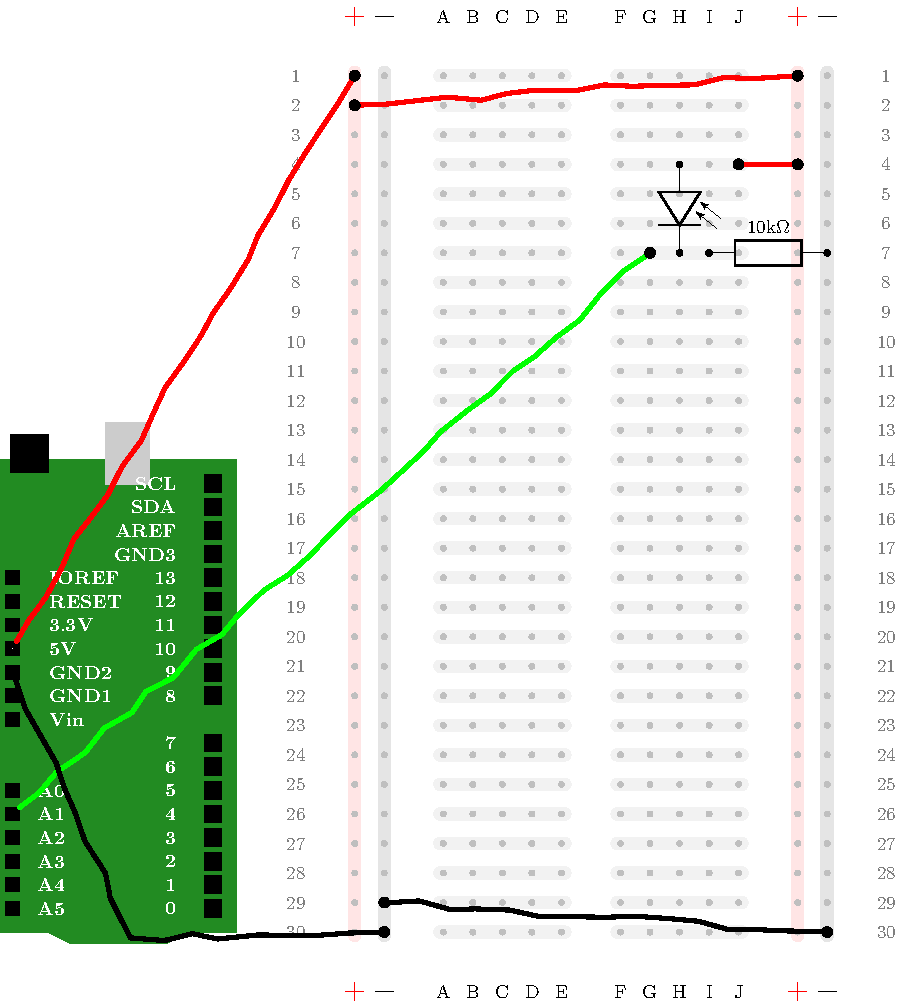
\includegraphics[width=0.8\textwidth]{kuvat/kuva14.pdf}


\begin{lstlisting}[numbers=none,showstringspaces=false]
void setup() {
  Serial.begin(9600);
}

void loop() {
  int valoan = analogRead(A1); // Luetaan anturin arvo portista A1
  Serial.print("Anturin arvo: "); // Selitys
  Serial.println(valoan); // ja tulostetaan se
  delay(1000); // Odotetaan, etta ehditaan lukea
}
\end{lstlisting}

\begin{tcolorbox}[colback=yellow!10, title={Valoanturin arvo},colbacktitle=orange]
Kirjoita ylös saamasi huoneen valoisuutta kuvaava arvo. Esimerkiksi 400.
\end{tcolorbox}

\subsection{LEDien lisääminen}\label{sec:valo}
\begin{minipage}{0.5\textwidth}
\begin{tcolorbox}[colback=lime!10,title=Tarvikkeet, colbacktitle=green!10,coltitle=black]
\begin{itemize}
    \item Edellisen kohdan piiri rakennettuna
    \item Sininen ja vihreä LED
    \item 2 kappaletta 220$\Omega$ vastuksia:   
\includegraphics[width=0.5\textwidth]{kuvat/220.pdf}
    \item Taskulamppu tai muu valonlähde
\end{itemize}
\end{tcolorbox}
\end{minipage}
\begin{minipage}{0.5\textwidth}
\begin{tcolorbox}[colback=blue!10,title=Piirin toiminta,colbacktitle=purple!90]
Lisätään havainnointia varten kaksi LEDiä, joilla saadaan tietää onko huoneessa valoisaa vai pimeää.
\tcblower
\begin{center}
\begin{tikzpicture}
\ctikzset{american}
\draw (0,4) to [led,l=vihreä,fill=green] (0,2);
\draw (0,2) to[R,a=$220\Omega$] (0,0);
\draw (0,0) -- (0,-0.5) node[ground]{}; 
\draw (-1,4) node[left] {4} to[short,o-] (0,4);

\draw (3,4) to [led,l=sininen,fill=blue] (3,2);
\draw (3,2) to[R,a=$220\Omega$] (3,0);
\draw (3,0) -- (3,-0.5) node[ground]{}; 
\draw (2,4) node[left] {5} to[short,o-] (3,4);

\end{tikzpicture}
\end{center}
\end{tcolorbox}
\end{minipage}

\begin{tcolorbox}[colback=red!10,colbacktitle=red,title=HUOM!]
Aina kun rakennat tai muutat piiriä, pidä Arduino irrotettuna tietokoneesta! 
\end{tcolorbox}

\clearpage
Lisätään LEDit sekä vastukset kuvan mukaisesti.

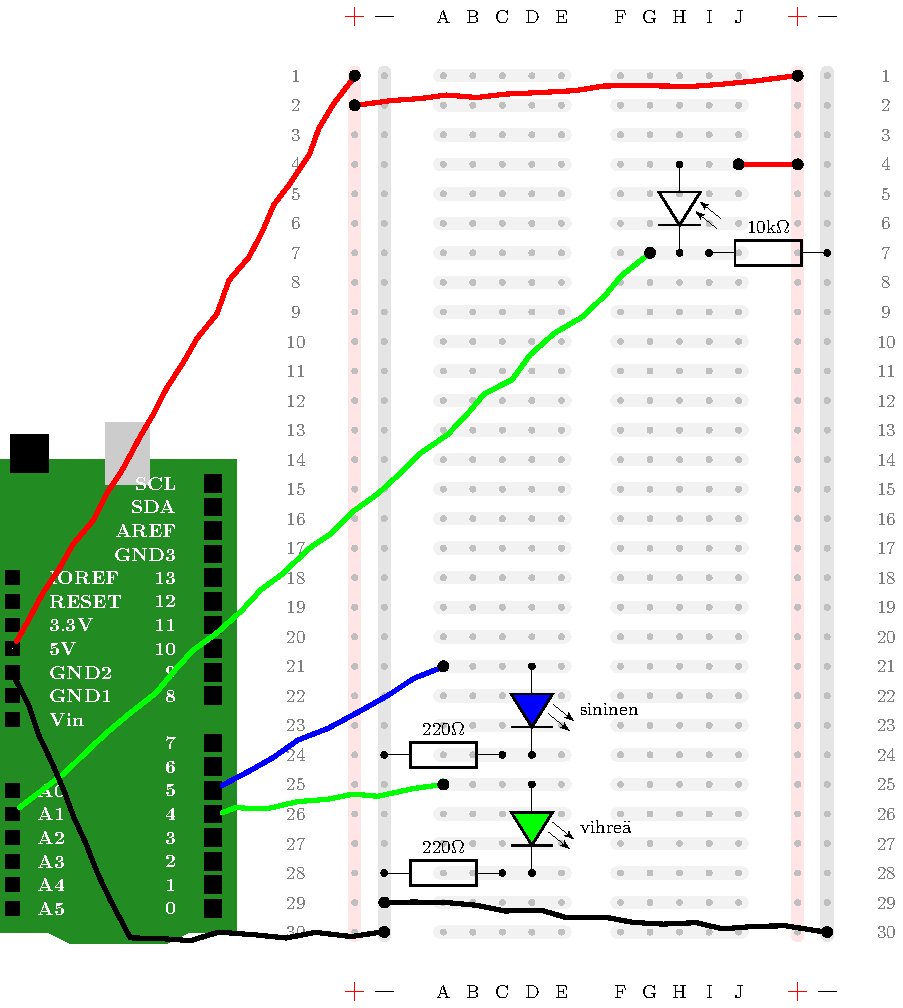
\includegraphics[width=0.9\textwidth]{kuvat/kuva15.pdf}
\clearpage
Lisätään taas LEDit koodiin. 
\begin{lstlisting}[numbers=none]
// Perusvalon aiheuttama lukema
int valo = 400; // Muokkaa arvoksi, jonka sait edellisesta tehtavasta

void setup() {
  Serial.begin(9600);
  pinMode(5,OUTPUT); // Sininen LED
  pinMode(4,OUTPUT); // Vihrea LED
}

void loop() {
  int valoan = analogRead(A1); // Luetaan anturin arvo portista A1
  Serial.print("Anturin arvo: "); // Selitys
  Serial.println(valoan); // ja tulostetaan se

  // Mita tehdaan? 
  if (valoan < valo){
    digitalWrite(5,HIGH); // Sytytetaan sininen valo
    digitalWrite(4,LOW); // Sammutetaan vihrea valo
  } else if (valoan >= valo && valoan < 2*valo) {
    digitalWrite(5,LOW); // Sammutetaan sininen valo
    digitalWrite(4,LOW); // Sammutetaan vihrea valo
  } else if (valoan>=2*valo) {
    digitalWrite(5,LOW); // Sammutetaan sininen valo
    digitalWrite(4,HIGH); // Sytytetaan vihrea valo
  }

  delay(1000); // Odotetaan, etta ehditaan lukea
}
\end{lstlisting}

\begin{tcolorbox}[colback=yellow!10, title={Tutki!},colbacktitle=orange]
Peitä kädellä valoanturi. Kumpi valo syttyy?

Lisää valoa esimerkiksi taskulampulla. Kumpi valo syttyy?

\begin{solution}
Sininen valo syttyy kun on pimeää ja vihreä kun on valoisaa.
\end{solution}
\end{tcolorbox}

\section{Valo- ja lämpöanturit}
\begin{minipage}{0.5\textwidth}
\begin{tcolorbox}[colback=lime!10,title=Tarvikkeet, colbacktitle=green!10,coltitle=black]
\begin{itemize}
    \item Edellisten kahden kohdan piirit (\ref{sec:lampo} ja \ref{sec:valo}) rakennettuna
\end{itemize}
\end{tcolorbox}
\end{minipage}
\begin{minipage}{0.5\textwidth}
\begin{tcolorbox}[colback=blue!10,title=Piirin toiminta,colbacktitle=purple!90]
Yhdistetään valo- ja lämpöanturit.
\end{tcolorbox}
\end{minipage}

\begin{tcolorbox}[colback=red!10,colbacktitle=red,title=HUOM!]
Aina kun rakennat tai muutat piiriä, pidä Arduino irrotettuna tietokoneesta! 
\end{tcolorbox}

Jos sinulla on edelleen jäljellä kohtien \ref{sec:lampo} ja \ref{sec:valo} piirit, sinulla pitäisi olla seuraavan sivun kuvan mukaiset kytkennät. Jos olet kuitenkin purkanut osan piireistä, kokoa se uudelleen kuvan mukaisesti.

\begin{tcolorbox}[title=Haaste!,colback=teal!10,colbacktitle=teal!90]
Suunnittele oma hälytysjärjestelmä, joka reagoi joko valon tai lämmön tai molempien muutoksiin.
\tcblower
Seuraavana on kuva, jossa on yhdistetty molemmat piirit ja sitä seuraa koodi, joka yhdistää jo tekemämme koodit. Voit käyttää sitä pohjana suunnitelmallesi.

\end{tcolorbox}

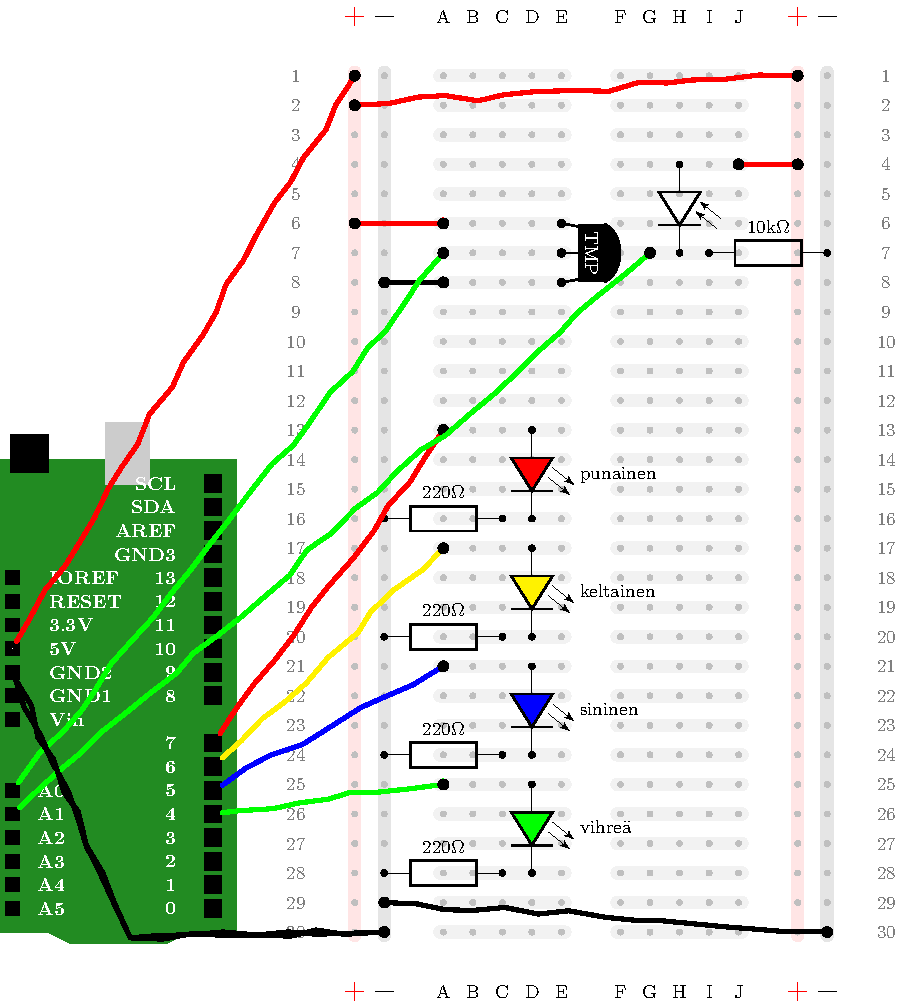
\includegraphics[width=0.95\textwidth]{kuvat/kuva16.pdf}

\begin{lstlisting}[numbers=none]
// Huoneen normaalit lukemat
int valo = 400; // Muokkaa saamaksesi arvoksi
const float huoneLamp = 20.0; // Muokkaa saamaksesi arvoksi

void setup() {
  Serial.begin(9600);
  pinMode(7,OUTPUT); // Punainen LED
  pinMode(6,OUTPUT); // Keltainen LED
  pinMode(5,OUTPUT); // Sininen LED
  pinMode(4,OUTPUT); // Vihrea LED
}

void loop() {
  int valoan = analogRead(A1); // Luetaan valoanturin arvo portista A1
  Serial.print("Valoanturin arvo: "); // Selitys
  Serial.println(valoan); // ja tulostetaan se
  
  int sensorVal = analogRead(A0); // Luetaan anturin arvo portista A0
  Serial.print("Lampotila: "); // lisataan selitys luvulle
  float voltage = (sensorVal/1024.0)*5.0; // Muunna anturin arvo volteiksi
  float temp = (voltage-0.5)*100;  // Muunnetaan jannite Celcius-asteiksi
  Serial.print(temp); // ja tulostetaan lampotila
  Serial.println(" C."); // Celcius-astetta ja vaihdetaan rivia

  // Mita tehdaan? 
  if (valoan < valo){
    digitalWrite(5,HIGH); // Sytytetaan sininen valo
    digitalWrite(4,LOW); // Sammutetaan vihrea valo
  } else if (valoan >= valo && valoan < 2*valo) {
    digitalWrite(5,LOW); // Sammutetaan sininen valo
    digitalWrite(4,LOW); // Sammutetaan vihrea valo
  } else if (valoan>=2*valo) {
    digitalWrite(5,LOW); // Sammutetaan sininen valo
    digitalWrite(4,HIGH); // Sytytetaan vihrea valo
  }

  if (temp < huoneLamp-2){
    // Huoneessa alkaa olla kylma
    digitalWrite(7,LOW); // Sammutetaan punainen LED tarvittaessa
    digitalWrite(6,HIGH); // Sytytetaan keltainen LED
  }else if(temp>=huoneLamp-2 && temp <huoneLamp+2){
    // Normaalihuoneen lampo
    digitalWrite(7,LOW); // Sytytetaan punainen valo
    digitalWrite(6,LOW); // Sytytetaan keltainen valo
  }else if (temp>huoneLamp+2) {
    // Lampo on noussut liikaa, varoitetaan pelkalla punaisella valolla
    digitalWrite(7,HIGH); // Sytytetaan punainen valo
    digitalWrite(6,LOW); // Sammutetaan keltainen valo
  }
 
  delay(1000); // Odotetaan, etta ehditaan lukea
}
\end{lstlisting}



\begin{tcolorbox}[colback=yellow!10, title={Koodaa!},colbacktitle=orange,breakable]
\vspace{15cm}
\begin{solution}
%\vspace{15cm}

Tähän tehtävään ei ole malliratkaisua
\end{solution}
\end{tcolorbox}